\documentclass{article}
% --- watermark (auto-inserted) ---
\usepackage{xcolor}
\usepackage{xfp}% \fpeval; in the kernel since 2022, harmless on older LaTeX
\usepackage{draftwatermark}
\newlength{\watermarkTextWidth}
\AddToHook{begindocument/end}{%
  \SetWatermarkText{\normalfont Generated by The Agentic Scientist}%
  \SetWatermarkFontSize{10pt}%
  \SetWatermarkLightness{0.85}%
  \settowidth{\watermarkTextWidth}{\normalfont\fontsize{10pt}{12pt}\selectfont Generated by The Agentic Scientist}%
  \edef\watermarkScale{\fpeval{0.8 * sqrt(\paperwidth**2 + \paperheight**2) / \watermarkTextWidth}}%
  \edef\watermarkAngle{\fpeval{atand(\paperheight/\paperwidth)}}%
  \SetWatermarkScale{\watermarkScale}%
  \SetWatermarkAngle{\watermarkAngle}%
}
% --- end watermark ---

\usepackage{paper,times}
\usepackage{amsmath,amssymb,graphicx,booktabs,subcaption}
\usepackage{hyperref,url,placeins}
\hypersetup{hidelinks}
\title{Width and Delayed Generalization in Finite-Horizon Modular Addition}
\author{}
\newcommand{\fit}{t_{\mathrm{fit}}}
\newcommand{\gen}{t_{\mathrm{gen}}}
\begin{document}
\maketitle

\begin{abstract}
Increasing model width can accelerate training-set fitting without improving generalization on the same training budget. We examine this distinction in modular addition using a fixed two-embedding network, a common optimizer configuration, and paired zero-decay and initial-norm controls. In the short-horizon development data, increasing hidden width from 32 to 256 reduces sustained fitting onset from 2,200--2,800 to 200 updates, yet held-out endpoint accuracy is nonmonotone in width. In a separate, longer-horizon final evaluation, the two retained width-128 trajectories exhibit delayed generalization, whereas three width-32 trajectories remain right-censored. Only five of nine planned width--seed records are available; no width-256 final record is retained. The final evaluation completed but failed scientific qualification, with no diagnostic identifying the cause. These observations support a conditional distinction between fitting speed and finite-horizon generalization, not a qualified model-size law. Initial-global-norm matching and zero-decay comparisons constrain simple interpretations but do not identify a mechanism or resolve missing outcomes.
% @evidence[[paper_data.json#/best_correct/evaluation_evidence/episodes]]
% @evidence[[paper_data.json#/final_evaluation/evaluation_evidence/episodes]]
% @evidence[[paper_data.json#/final_evaluation/outcome]]
\end{abstract}

\section{Introduction}
The time needed to fit a training set need not predict the time needed to generalize. Small algorithmic datasets make this distinction especially clear: a neural network can achieve nearly perfect training accuracy while its performance on unseen inputs remains poor, and only much later improve. This phenomenon, termed grokking by \citet{Power2022GrokkingGB}, provides a controlled setting in which optimization, memorization, and generalization can be examined separately. Model size is a natural experimental variable, but its interpretation requires care. A wider network changes representational capacity, initialization geometry, and optimization simultaneously. Earlier fitting alone does not demonstrate an earlier discovery of the underlying algorithm.

We ask how hidden width relates to training-fit onset and held-out generalization in a fixed modular-addition architecture. Our working explanation is deliberately operational: width can shorten the fitting timescale without shortening the timescale for a well-generalizing solution enough to be observable at a fixed horizon. A simple alternative predicts that increasing width should improve both fitting speed and held-out endpoint accuracy under the same training budget. The available comparisons test that monotone prediction directly. They do not measure the internal computation needed to turn a timescale separation into a causal theory.

The study varies width while retaining the task, model family, loss, and common optimizer settings. Matched comparisons include a fixed reference configuration, removal of weight decay, and rescaling to a common initial global parameter norm. Short-horizon data contain complete paired width comparisons; the longer-horizon final data have incomplete width coverage. We keep these evidence sets separate because their seeds, input pools, and training horizons differ. Their contrast cannot be interpreted as an intervention on training duration alone.

The main empirical finding is a dissociation: larger widths fit earlier in the development data, but held-out accuracy is not monotone in width. Two retained intermediate-width final trajectories show substantial delays between fitting and generalization. However, the final evaluation completed without scientific qualification. Its missing qualification diagnostics do not establish whether the failure arose from performance, uncertainty, validity, adaptivity, or another criterion. Incomplete observations are a documented limitation, not an explanation of that failure.
% @evidence[[paper_data.json#/final_evaluation]]

Our contributions are a source-linked comparison of fitting and generalization across the measured widths, a control-aware interpretation that separates actual interventions from duplicated conditions, and a censoring-aware account of what remains unidentified. These are bounded empirical contributions. We neither introduce a new optimizer nor claim a scaling law, statistical superiority, a circuit explanation, or a validated decay-clock mechanism. The value of the study lies in distinguishing observations that survive close inspection from stronger conclusions that the available design cannot support.

\begin{figure}[t]
\centering
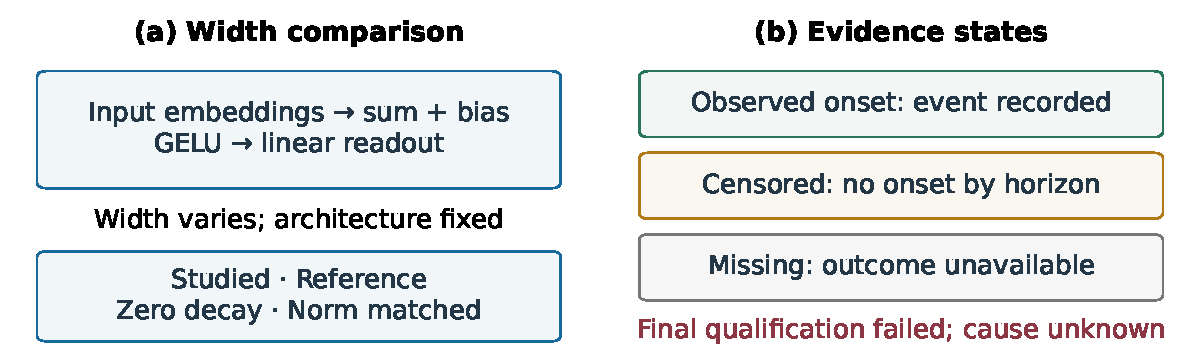
\includegraphics[width=\textwidth]{figures/study_overview.pdf}
\caption{Design and observation states, not a mechanistic explanation. Width varies within a fixed modular-addition network and paired control conditions. A recorded generalization onset, a trajectory censored at the observation horizon, and an unavailable record are distinct evidence states. None overrides the failed final scientific qualification.}
\label{fig:overview}
\end{figure}
% @evidence[[source_evidence/task/evaluate_final.py#L801]]
% @evidence[[paper_data.json#/final_evaluation/evaluation_evidence/episodes]]
% @evidence[[paper_data.json#/grounding_sources/final.qualification.outcome]]

\section{Related Work}
\paragraph{Algorithmic generalization and internal progress.}
\citet{Power2022GrokkingGB} established small algorithmically generated datasets as a setting for generalization well after training-set fitting. \citet{Nanda2023Progress} reverse-engineered a Fourier-based algorithm in small Transformers trained on modular addition and developed progress measures based on that computation. Our network instead sums learned input embeddings before a GELU and a linear readout. We measure threshold onsets and endpoint behavior, not Fourier circuits or representation-specific progress. Consequently, architectural or mechanistic conclusions from those Transformers are not evidence for the internal computation of the present network.

\paragraph{Norm, efficiency, and feature learning.}
\citet{Liu2022OmnigrokGB} relate grokking to training and test loss landscapes as a function of weight norm. \citet{Varma2023ExplainingGT} explain delayed generalization through competition between memorizing and generalizing circuits with different norm efficiency and learning speed. \citet{Kumar2023GrokkingAT} study a lazy-to-rich transition, including polynomial regression in which delayed generalization occurs without weight decay. These accounts motivate different diagnostics: initial norm, efficiency of task-relevant computations, and evolving features are not interchangeable quantities. Our norm-rescaling and zero-decay controls address limited observable consequences. They do not measure circuit efficiency, kernel alignment, or the onset of feature learning, and cannot select among these explanations.

\paragraph{Capacity and duration.}
\citet{Davies2023Unifying} propose a pattern-learning-speed framework connecting grokking and double descent, including changes in model capacity. \citet{Nakkiran2020Double} show that model size and training duration can each produce nonmonotone test behavior. These works motivate joint attention to width and observation horizon, rather than an assumption that larger networks must generalize better at every endpoint. Our narrow width sweep is not an estimate of a double-descent curve. Finally, AdamW decouples weight decay from the adaptive loss-gradient update \citep{Loshchilov2019AdamW}. Matching the nominal decay factor is therefore a useful optimizer description, not proof of equal effective regularization or equal post-fit exposure.

\section{Method}
\subsection{Problem Setup and Evaluation Target}
The task is classification of $y=(a+b)\bmod p$ for integer residues $a,b\in\{0,\ldots,p-1\}$ with $p=97$. The full domain contains $p^2$ ordered input pairs. The supplied development and final resources partition that domain into disjoint pools of 4,704 and 4,705 inputs. Each seed defines a training/evaluation split within its pool, with training fraction 0.6. Development splits contain 2,822 training and 1,882 evaluation examples; final splits contain 2,823 and 1,882, respectively. The fixed pools and seed-specific splits, rather than the full operation table, define the measured generalization target. No additional task with recorded results is present.
% @evidence[[source_evidence/task/resources/search/dataset.json#/pool_size]]
% @evidence[[source_evidence/task/resources/final/dataset.json#/splits]]
% @evidence[[paper_data.json#/best_correct/evaluation_evidence/episodes]]

For hidden width $w$, the logits are
\begin{equation}
 z_\theta(a,b)=\operatorname{GELU}\!\left(E^{(1)}_{a,:}+E^{(2)}_{b,:}+c\right)W+d,
 \label{eq:model}
\end{equation}
where $E^{(1)},E^{(2)}\in\mathbb{R}^{p\times w}$, $c\in\mathbb{R}^{w}$, $W\in\mathbb{R}^{w\times p}$, and $d\in\mathbb{R}^{p}$. Full-batch cross-entropy is minimized using AdamW in float32 on CPU. Widths are $32,128,256$, with $292w+97$ trainable parameters: 9,441, 37,473, and 74,849. All biases start at zero. The model has no attention, recurrence, or depth intervention. The inspected final training source implements this architecture directly (Supplementary Information, Section~\ref{sec:source}).
% @evidence[[source_evidence/task/evaluate_final.py#L801]]
% @evidence[[derived/observations.json#/rows]]

\subsection{Hypotheses and Interventions}
We distinguish two observable predictions. A \emph{monotone width-benefit prediction} expects earlier fitting and no reduction in held-out endpoint accuracy as width increases at fixed training horizon. A \emph{separated-timescale explanation} allows earlier fitting alongside worse short-horizon generalization; it predicts that fitting onset alone will not order held-out performance. A stronger claim that width systematically shortens the post-fit delay would require comparable, observed generalization onsets across widths. Our evidence can challenge the monotone prediction but cannot establish that stronger claim.

Initialization is coupled by seed across widths: Gaussian embedding and readout tensors are drawn at the maximum width, then sliced. Embeddings are multiplied by a common multiplier $m$, and the readout is scaled by $m/\sqrt{w}$. This pairing reduces arbitrary initialization differences without making different widths functionally equivalent. The studied condition uses learning rate $\eta=0.003$, weight decay $\lambda=1.0$, and $m=0.5$. It is common across widths and seeds, not adapted using training curves. It was selected using development evaluations; those observations therefore remain selection-conditioned rather than confirmatory.
% @evidence[[source_evidence/task/evaluate_final.py#L803]]
% @evidence[[source_evidence/controllers/studied/src/program.py#L37]]
% @evidence[[paper_data.json#/best_correct/evaluation_evidence/episodes]]

Each retained width--seed cell contains the following matched conditions:
\begin{itemize}
\item \textbf{Studied:} the common configuration above.
\item \textbf{Reference:} $\eta=0.001$, $\lambda=1.0$, $m=1.0$, with the same width, seed, split, and horizon. Because both learning rate and initialization differ, this is a configuration comparison, not a component-specific test.
\item \textbf{No decay:} the studied configuration with $\lambda=0$. This isolates removal of decay within the measured setting, not its necessity for all delayed generalization.
\item \textbf{Norm matched:} the studied initialization is rescaled so its global Euclidean parameter norm equals that of the same-seed width-128 initialization. Learning rate and decay are unchanged. This matches one scalar, not capacity, layerwise geometry, or initial function.
\end{itemize}
% @evidence[[source_evidence/task/evaluate_final.py#L795]]
% @evidence[[source_evidence/task/evaluate_final.py#L821]]
At width 128 the norm-matching target is the original model itself. The retained initial/final state hashes and scientific metric trajectories match the studied condition there. This duplicate supplies neither an independent replication nor an additional delayed event.
% @evidence[[paper_data.json#/final_evaluation/evaluation_evidence/episodes]]

\subsection{Training Protocol and Event Definitions}
Development observations use seeds 101 and 211 and a horizon of 6,000 updates. Final observations use seeds 60613, 70717, and 80821 with a planned horizon of 24,000 updates. Accuracy is recorded at initialization and every 100 updates. All four conditions in a retained cell use the same split. Distinct development/final pools prevent exact input overlap across those resources, but the longer final horizon also changes alongside the seeds and data. No paired duration-only contrast is available.
% @evidence[[paper_data.json#/best_correct/evaluation_evidence/episodes]]
% @evidence[[paper_data.json#/final_evaluation/evaluation_evidence/episodes]]

For a checkpoint accuracy sequence $A(t)$, define a sustained threshold onset as
\begin{equation}
 T_q[A]=\min\{t_j:\ A(t_j),A(t_{j+1}),A(t_{j+2})\geq q\},
 \qquad
 \fit=T_{0.99}[A_{\mathrm{train}}],\quad
 \gen=T_{0.95}[A_{\mathrm{eval}}].
 \label{eq:onset}
\end{equation}
The onset is the first checkpoint in the qualifying triplet, not the confirmation time. When both onsets exist, the delay is $\max(0,\gen-\fit)$. A delayed event requires a delay of at least 1,000 updates. If either onset is absent, the evaluator records censoring and a normalized capped-delay value of one. This last convention is a reporting functional, not an observed event time. Three consecutive checkpoints suppress single-checkpoint spikes but do not guarantee persistent accuracy after the qualifying window. We retain the distinction between threshold-defined delayed generalization and a mechanistically verified transition.
% @evidence[[source_evidence/task/evaluate_final.py#L1001]]
% @evidence[[paper_data.json#/final_evaluation/evaluation_evidence/episodes]]

\subsection{Reporting, Missingness, and Uncertainty}
The unit of replication is the seed, not the evaluation example, checkpoint, or matched condition. We report all retained seed values and descriptive sample standard deviations where appropriate. Paired differences use only seeds shared by the compared widths. We do not replace the planned widest-minus-narrowest final contrast with an intermediate-minus-narrowest contrast without explicitly naming that change in estimand. Missing width records have no performance outcome; they are not measured losses, censored trajectories, or zero-accuracy models.

For transparency, we also give exact binomial intervals for delayed-event counts conditional on retained records. These intervals describe what a hypothetical independent-seed sampling model would allow; the small sample and unknown missingness preclude a population interpretation. No inferential test uses examples or checkpoints as extra replications. Failed final qualification applies independently of these descriptive calculations. The final summary supplies no criterion-specific diagnostics, so neither the observed missingness nor the retained controls can certify validity or identify the cause of non-qualification.
% @evidence[[paper_data.json#/final_evaluation/limitations]]
% @evidence[[derived/summary.json#/cells]]

\section{Results}
\subsection{Evidence Coverage and Scientific Qualification}
Table~\ref{tab:coverage} gives the full final observation pattern for the studied condition. Only five of nine planned width--seed cells are retained: three at width 32, two at width 128, and none at width 256. All retained cells contain complete-horizon trajectories for the matched conditions. At width 32, failure to observe the sustained generalization threshold is right censoring at the recorded horizon. At width 256, absence of trajectories provides no information about onset or endpoint accuracy. The missing width-128 seed is likewise unavailable, not evidence against generalization.
% @evidence[[paper_data.json#/final_evaluation/evaluation_evidence/episodes]]

\begin{table}[t]
\centering
\caption{Final coverage for the studied condition. C: recorded trajectory, generalization onset censored at 24,000 updates; D: recorded delayed event; M: missing record. A missing cell is not assigned an accuracy or a censoring time. All conditions in each retained cell were recorded.}
\label{tab:coverage}
\begin{tabular}{lccc}
\toprule
Seed & Width 32 & Width 128 & Width 256 \\
\midrule
60613 & C & D & M \\
70717 & C & D & M \\
80821 & C & M & M \\
\bottomrule
\end{tabular}
% @evidence[[paper_data.json#/final_evaluation/evaluation_evidence/episodes]]
\end{table}

The final evaluation completed but did not qualify. We preserve that conclusion rather than interpreting selection as scientific acceptance. No supplied diagnostic distinguishes a statistical/performance failure from a validity or adaptivity failure. Retained observations can describe the measured trajectories, but they cannot restore claims that would require qualification. In particular, neither complete trajectories in individual cells nor successful execution of local controls establishes general validity of the final comparison.
% @evidence[[paper_data.json#/grounding_sources/final.qualification.status]]
% @evidence[[paper_data.json#/grounding_sources/final.qualification.outcome]]
% @evidence[[paper_data.json#/grounding_sources/final.qualification.correct]]

\subsection{Width Accelerates Fitting but Does Not Order Short-Horizon Accuracy}
The short-horizon comparisons show a consistent fitting order. In the studied condition, width-32 fitting onsets are 2,200 and 2,800 updates; width 128 fits at 300 updates in both seeds; width 256 fits at 200 in both seeds. The paired widest-minus-narrowest differences are thus $-2,000$ and $-2,600$ updates. Yet held-out endpoint accuracy is highest at width 32, lowest at width 128, and intermediate at width 256 in each seed (Table~\ref{tab:development}, Figure~\ref{fig:endpoint}). Earlier training fit therefore does not order generalization at this horizon.
% @evidence[[derived/summary.json#/cells]]
% @evidence[[derived/summary.json#/paired/development_256_minus_32]]

\begin{table}[t]
\centering
\caption{Studied condition at the 6,000-update development horizon. Accuracy is mean $\pm$ sample SD over the two seeds, in percent. Onsets are listed by seed rather than averaged with unobserved values. No sustained held-out onset is observed at any width.}
\label{tab:development}
\begin{tabular}{lrrr}
\toprule
Width & Parameters & Training-fit onsets & Held-out accuracy (\%) \\
\midrule
32 & 9,441 & 2,200; 2,800 & $74.68\pm4.47$ \\
128 & 37,473 & 300; 300 & $29.33\pm3.68$ \\
256 & 74,849 & 200; 200 & $39.35\pm3.49$ \\
\bottomrule
\end{tabular}
% @evidence[[derived/summary.json#/cells]]
% @evidence[[derived/observations.json#/rows]]
\end{table}

The monotone width-benefit prediction is contradicted by these measured endpoints. This does not refute every possible benefit of width: intermediate held-out performance may depend on the optimization path, and the observation horizon may precede a later transition. Nor does the pattern establish a double-descent curve, which would require a broader sweep and a justified interpolation-regime interpretation. The supported statement is narrower: a shared training budget and common optimizer settings do not make greater width synonymous with better held-out accuracy in these development observations.

\begin{figure}[t]
\centering
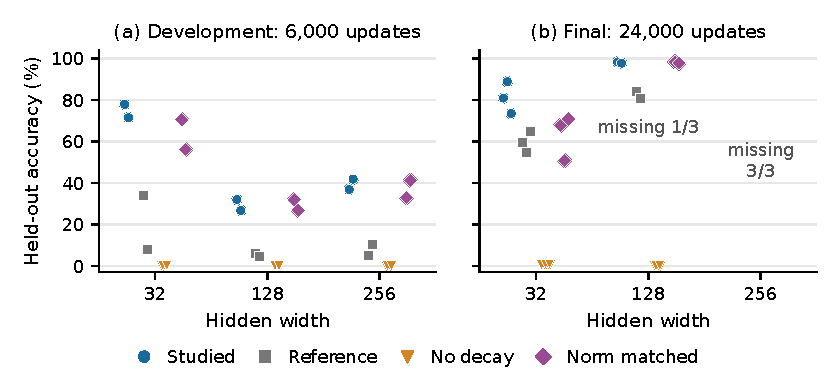
\includegraphics[width=\textwidth]{figures/width_endpoint_comparison.pdf}
\caption{Matched-condition endpoint comparisons. (a) Development observations at 6,000 updates. (b) Retained final observations at 24,000 updates. Each dot is a recorded seed; no missing cell is plotted at zero. The panels use different seeds and disjoint input pools, so their contrast is not a duration-only intervention. At width 128, norm matching duplicates the studied scientific trajectory; horizontally separated symbols do not denote independent evidence.}
\label{fig:endpoint}
% @evidence[[derived/observations.json#/rows]]
\end{figure}

\subsection{Retained Delayed Events at Intermediate Width}
At the final horizon, the two retained width-128 studied trajectories first fit at 300 and 200 updates and first satisfy the sustained held-out threshold at 17,600 and 19,200 updates, respectively. Their observed delays are therefore 17,300 and 19,000 updates. Their endpoints are 98.353\% and 97.768\%. In contrast, width-32 fitting onsets are 2,600, 2,400, and 3,000 updates, with no sustained held-out onset by 24,000 updates; endpoints are 80.925\%, 88.842\%, and 73.433\%. Figure~\ref{fig:onsets} separates these delayed events from right censoring and missing records.
% @evidence[[paper_data.json#/final_evaluation/evaluation_evidence/episodes]]
% @evidence[[derived/observations.json#/rows]]

For the two shared final seeds, width-128 minus width-32 endpoint differences are 17.428 and 8.927 percentage points. This is a conditional intermediate-versus-narrow comparison. The widest-versus-narrowest final comparison is unavailable, and all final seed-level contrasts requiring the complete width set are absent from the supplied summary. It would be inappropriate to present the retained intermediate-width advantages as a complete ordering of model sizes or an estimate of a general width effect.
% @evidence[[derived/summary.json#/paired/final_128_minus_32]]
% @evidence[[paper_data.json#/final_evaluation/evaluation_evidence/episodes]]

Conditional on the retained records, the delayed-event counts are two of two at width 128 and zero of three at width 32. Exact 95\% binomial intervals are approximately $[0.158,1]$ and $[0,0.708]$. These wide intervals make the uncertainty visible even under an independent-seed assumption; missingness and failed qualification impose additional limits that such intervals do not repair. They are neither a significance result nor evidence that width-32 models can never generalize. The design-weighted final event fraction, two of nine, uses a different denominator and must not be confused with either conditional fraction.
% @evidence[[derived/summary.json#/cells/final_128]]
% @evidence[[derived/summary.json#/cells/final_32]]
% @evidence[[paper_data.json#/grounding_sources/final.metric.grokking_incidence]]

\begin{figure}[t]
\centering
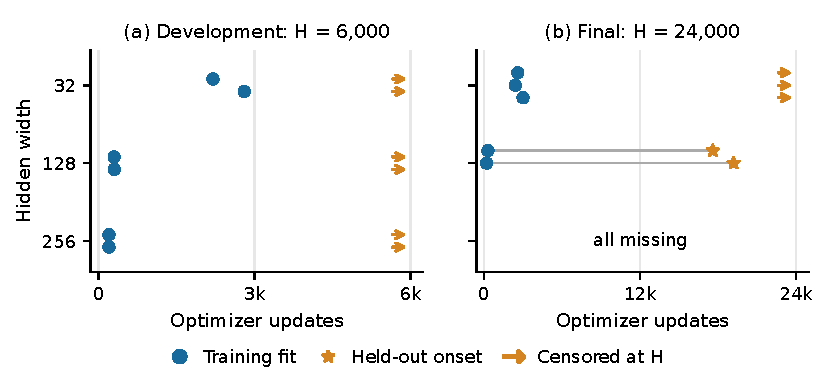
\includegraphics[width=\textwidth]{figures/fit_and_generalization_onsets.pdf}
\caption{Training-fit and held-out onsets for the studied condition. Each vertical offset identifies a seed within a width. A circle is sustained training fit; a star is sustained held-out onset; an arrow indicates a recorded trajectory whose held-out onset is censored at the horizon. Missing trajectories receive no arrow. Onsets require three consecutive checkpoints at 0.99 training or 0.95 held-out accuracy. Panel axes deliberately differ because the horizons differ.}
\label{fig:onsets}
% @evidence[[derived/observations.json#/rows]]
% @evidence[[source_evidence/task/evaluate_final.py#L1001]]
\end{figure}

\subsection{What the Matched Controls Do and Do Not Explain}
Removing decay produces strong training/evaluation separation within the measured budget. In the retained final no-decay controls, width-32 held-out endpoints range from 0.478\% to 0.797\%, and both width-128 endpoints are zero. Nevertheless, training-fit onsets are 1,300--1,600 updates at width 32 and 200 updates at width 128. These measured configuration contrasts support a substantial finite-horizon difference between training fit and generalization with and without decay. They do not establish that weight decay is necessary for grokking in another architecture, task, optimizer, or training horizon.
% @evidence[[derived/observations.json#/rows]]

Global initial-norm matching does not eliminate the short-horizon narrow-versus-intermediate ordering: width-32 endpoints are 70.510\% and 56.164\%, compared with 31.934\% and 26.727\% at width 128. This challenges the limited proposal that matching this scalar alone would remove that observed ordering. It does not isolate a causal norm mediator. The intervention changes all nonzero initial parameter magnitudes together, while width still changes capacity and feature geometry. At width 128 it makes no change at all, so its delayed events duplicate the studied observations rather than independently confirming a norm explanation.
% @evidence[[paper_data.json#/best_correct/evaluation_evidence/episodes]]
% @evidence[[paper_data.json#/final_evaluation/evaluation_evidence/episodes]]

The retained final reference controls also do not cross the sustained held-out threshold. Their endpoints range from 54.570\% to 65.037\% at width 32 and from 80.659\% to 84.272\% at width 128. These are matched reference-configuration observations, not an attribution to initialization or learning rate alone. Together the controls narrow interpretation: they show that early fitting can coexist with poor held-out endpoints, and that scalar norm matching does not make width interchangeable. They do not reveal why delayed generalization occurs in the two retained intermediate-width trajectories.
% @evidence[[derived/observations.json#/rows]]

\subsection{Endpoint Norms and Losses Bound a Scalar-Clock Interpretation}
Accuracy-based fitting is not equivalent to convergence of the training objective. Every retained final studied trajectory ends at perfect training accuracy, but the corresponding cross-entropy losses differ substantially across widths (Table~\ref{tab:normloss}). The narrow models retain nonzero training loss even after their accuracy threshold has been exceeded; the intermediate-width models have much smaller final training losses. A statement about the time to classify the training set therefore should not be silently replaced by a statement about optimization completion, margin growth, or the time at which regularization becomes dominant.
% @evidence[[derived/observations.json#/rows]]

\begin{table}[t]
\centering
\caption{Endpoint diagnostics for all retained final studied trajectories. Norms are global Euclidean parameter norms; losses are cross-entropy at 24,000 updates. All listed endpoint training accuracies equal one. Net norm increases coexist with both observed and censored held-out onsets. No width-256 diagnostic is available.}
\label{tab:normloss}
\small
\begin{tabular}{rrrrrr}
\toprule
Seed & Width & Initial norm & Final norm & Train loss & Held-out loss \\
\midrule
60613 & 32 & 40.45 & 93.97 & 0.202 & 0.935 \\
60613 & 128 & 79.18 & 128.10 & 5.6e-05 & 0.110 \\
70717 & 32 & 40.31 & 94.18 & 0.178 & 0.703 \\
70717 & 128 & 79.34 & 128.31 & 5.78e-05 & 0.137 \\
80821 & 32 & 39.76 & 94.44 & 0.199 & 1.064 \\
\bottomrule
\end{tabular}
% @evidence[[derived/norm_loss_records.tex]]
\end{table}

Global norms increase between initialization and the final checkpoint in every retained studied record, including the delayed-event records. Thus, a positive weight-decay coefficient cannot be read as evidence of a net decline in the measured total norm. These endpoint comparisons do not establish monotonic norm growth during training, nor do they refute explanations based on relative circuit efficiency or trajectories through a loss landscape. A generalizing computation could become more efficient while the total norm still rises. The diagnostics instead expose the gap between an optimizer-level shrinkage term and a measured model-level explanation: the adaptive loss-gradient update and the decay update act together, while our evidence does not isolate their contributions to the learned computation.
% @evidence[[derived/observations.json#/rows]]

\section{Discussion and Limitations}
\subsection{A Conditional Timescale Distinction, Not a Size Law}
The cleanest interpretation is that training fit and useful generalization are separate empirical targets. In the complete short-horizon width comparisons, fitting accelerates while endpoint generalization does not improve monotonically. In the incomplete final comparisons, observed intermediate-width events are compatible with a long separation after fitting. These observations support the working explanation at a descriptive level. They do not tell us whether a wider model changes the formation, competition, or efficiency of task-relevant computations. A claim about any of those mechanisms would need corresponding measurements rather than a reinterpretation of accuracy alone.

The development/final contrast illustrates why observation horizon must be part of a statement about width. It does not show that extending training caused a reversal of the width ranking, since data and seeds also changed. Likewise, the fact that both observed delayed events occur at the intermediate width does not locate an optimal width: the largest width is missing entirely in the final data. Treating absence of the largest models as a negative outcome would manufacture the very comparison needed for that conclusion.

The no-decay results should be interpreted within the same boundary. AdamW applies a nominal multiplicative shrinkage factor of $1-\eta\lambda$ per update, alongside an adaptive gradient update. This factor is not a complete dynamical clock. Models may fit at different times, have different gradient histories, and accumulate different post-fit exposure even when this factor agrees. No positive-decay factorial grid, clock-collapse analysis, or direct efficiency measurement was completed in the retained evidence. A nominal optimizer relationship cannot substitute for those missing tests.
% @evidence[[source_evidence/task/evaluate_final.py#L833]]
% @evidence[[paper_data.json#/all_programs]]

\subsection{Validity, Selection, and Missing Information}
The final qualification failure is a substantive boundary on interpretation. No supplied criterion-level diagnosis establishes that the failure was merely insufficient performance, merely statistical uncertainty, or a protocol defect. Reporting the retained trajectories does not alter that status. Their source-linked availability permits inspection and reproduction of descriptive calculations; it does not certify all scientific conclusions one might wish to draw from them. The same caution applies to provenance hashes: matching source identity helps locate the evaluated implementation, but the readable implementation and actual observations, not the hash alone, support its substantive description.

Development observations were used to select the common configuration. Their apparent advantages over the fixed reference are therefore not an unbiased assessment of a newly chosen setting. The final data provide a separate evaluation, but missing cells prevent the planned complete-width contrasts, and its non-qualification prevents presenting it as a successful confirmation. Incomplete alternative configurations are preserved in the supplement rather than converted into measured losses or a retrospective success narrative.

Uncertainty is limited by the number of independent seeds, not by the number of labeled pairs. Seed-specific splits and coupled initialization make pairing useful, but also mean that each seed jointly varies multiple stochastic ingredients. We do not separately identify split uncertainty and initialization uncertainty. The retained records do not justify an assumption that missing cells are random. Consequently, complete-case endpoint differences, exact event-count intervals, and descriptive standard deviations must remain conditional summaries, not missing-data corrections or population guarantees.

The setting is also narrow: a single modular operation and modulus, a particular shallow architecture, fixed full-batch optimization, and a fixed observation rule. We did not measure random-label controls, frozen features, circuit ablations, additional moduli, or transfer to other tasks. No claim extends to those unmeasured conditions. Even within this task, three-checkpoint onset is an operational marker rather than proof of a permanent or abrupt algorithmic change. The conclusion concerns the recorded thresholds and endpoints, not an unobserved internal transition.

\section{Conclusion}
Hidden width and delayed generalization cannot be summarized by training-fit speed alone. In the available modular-addition comparisons, increasing width accelerates sustained fitting while held-out accuracy remains nonmonotone at the short horizon. The retained longer-horizon data contain delayed events at the intermediate width and censored narrow-width trajectories, but omit all largest-width records and one intermediate-width seed. These findings support a bounded separation between fitting and finite-horizon generalization, not a qualified scaling law.

The controls make that boundary more informative. Removing decay preserves rapid fitting without comparable held-out performance in the measured setting; matching initial global norm does not remove the observed development ordering and is exactly redundant at the matching width. Neither result identifies the mechanism of delayed generalization. Most importantly, the final evaluation failed scientific qualification, and its cause remains unspecified. A source-linked descriptive account is therefore the appropriate endpoint of this evidence: report the observed comparisons, distinguish censoring from missingness, and leave broad width effects and causal explanations unresolved.

\FloatBarrier
\clearpage
\bibliographystyle{paper}
\bibliography{references}
\clearpage
\appendix
\section{Supplementary Information}

\subsection{Inspectable Implementation and Data Resources}
\label{sec:source}
The included training implementation is \path{source_evidence/task/evaluate_final.py}. Architecture, initialization coupling, norm matching, and optimizer construction appear at lines 781--835; checkpoint measurement and local controls at lines 869--913; sustained-onset extraction at lines 1001--1016; and paired-width contrasts at lines 1074--1093. Its SHA-256 equals the final evaluator digest recorded in the evidence registry. This exact source check supplements, rather than replaces, inspection of the readable training code. Source and resource hashes are recorded in \path{derived/source_manifest.json}. The local controller snapshot is in \path{source_evidence/controllers/studied/}; its readable response specifies the common settings and agrees with every retained studied configuration. We do not claim an independent reconstruction of the complete frozen source tree from a tree digest.
% @evidence[[source_evidence/task/evaluate_final.py#L781]]
% @evidence[[derived/source_manifest.json]]
% @evidence[[paper_data.json#/final_evaluation/evaluator_sha256]]

The two data resources are \path{source_evidence/task/resources/search/dataset.json} and \path{source_evidence/task/resources/final/dataset.json}. They include the explicit integer triples, source-row identities, seed-specific train/evaluation indices, and split digests. All labels are verified by modular addition in the supplied evaluator. No third-party dataset download, account, license, or external snapshot is needed. Although the task domain is exhaustively enumerable, training and evaluation use the resource pools and their recorded splits, not an assumed random partition of the complete domain at each width. The partition is shared across widths within a seed.
% @evidence[[source_evidence/task/evaluate_final.py#L696]]
% @evidence[[source_evidence/task/resources/search/dataset.json]]
% @evidence[[source_evidence/task/resources/final/dataset.json]]

The reference uses the same seeded Gaussian draws as the studied model but a different initialization multiplier and learning rate. The norm-matched control rescales every parameter by the ratio of the same-seed width-128 norm to the current norm. Biases initially equal zero, so this is a global scaling of the nonzero embedding and readout tensors. It does not make individual layer norms equal across widths. Full-batch training leaves the optimizer's other settings at the pinned library defaults, with \texttt{foreach=False}; we do not infer additional tuning of unspecified optimizer parameters.
% @evidence[[source_evidence/task/evaluate_final.py#L795]]
% @evidence[[source_evidence/task/evaluate_final.py#L821]]

\subsection{Complete Retained Final Comparisons}
\begin{table}[h]
\centering
\caption{All retained final condition endpoints and onsets. S: studied; R: reference; Z: no decay; N: norm matched. Onset values are updates. The $>24000$ notation means no sustained held-out onset was recorded; it is not an extrapolated event time. All listed training onsets are observed. Missing width--seed cells are given separately in Table~\ref{tab:coverage}, not inserted as zero-valued rows.}
\label{tab:allfinal}
\small
\begin{tabular}{rrrrrr}
\toprule
Seed & Width & Arm & Accuracy (\%) & Fit & Onset \\
\midrule
60613 & 32 & S & 80.925 & 2600 & $>24000$ \\
60613 & 32 & R & 59.352 & 9100 & $>24000$ \\
60613 & 32 & N & 67.747 & 3400 & $>24000$ \\
60613 & 32 & Z & 0.478 & 1600 & $>24000$ \\
60613 & 128 & S & 98.353 & 300 & 17600 \\
60613 & 128 & R & 84.272 & 700 & $>24000$ \\
60613 & 128 & N & 98.353 & 300 & 17600 \\
60613 & 128 & Z & 0.000 & 200 & $>24000$ \\
70717 & 32 & S & 88.842 & 2400 & $>24000$ \\
70717 & 32 & R & 54.570 & 11100 & $>24000$ \\
70717 & 32 & N & 50.797 & 4500 & $>24000$ \\
70717 & 32 & Z & 0.744 & 1400 & $>24000$ \\
70717 & 128 & S & 97.768 & 200 & 19200 \\
70717 & 128 & R & 80.659 & 700 & $>24000$ \\
70717 & 128 & N & 97.768 & 200 & 19200 \\
70717 & 128 & Z & 0.000 & 200 & $>24000$ \\
80821 & 32 & S & 73.433 & 3000 & $>24000$ \\
80821 & 32 & R & 65.037 & 9600 & $>24000$ \\
80821 & 32 & N & 70.829 & 3400 & $>24000$ \\
80821 & 32 & Z & 0.797 & 1300 & $>24000$ \\
\bottomrule
\end{tabular}
% @evidence[[derived/observations.json#/rows]]
\end{table}

The full machine-readable record \path{derived/observations.json} also lists initial and final global norms, parameter counts, initial/final state hashes, updates, and recorded condition durations. It is deterministically extracted from the immutable evidence registry rather than a new evaluation. At width 128, comparison of initial and final hashes and the non-wall-time checkpoint metrics confirms the identity of the studied and norm-matched observations. Their runtime measurements need not coincide, so this identity concerns model states and scientific metrics, not elapsed time.
% @evidence[[derived/observations.json#/rows]]
% @evidence[[paper_data.json#/final_evaluation/evaluation_evidence/episodes]]

\subsection{Selection Sensitivity and Incomplete Settings}
The development evidence contains related common configurations with learning-rate/decay/initialization triples $(0.003,1.0,1.0)$, $(0.003,1.0,0.5)$, and $(0.006,0.5,0.5)$. These are sensitivity conditions, not independent scientific replications of the final comparison. The first two differ in initialization at fixed learning rate and decay. The last differs in learning rate and decay while preserving the nominal product $\eta\lambda$ relative to the studied condition. Equal products do not imply equal adaptive updates or effective regularization. Their full observations remain in the registry, and the controller snapshots are supplied with the code.
% @evidence[[paper_data.json#/all_programs/0/evaluation_evidence/episodes]]
% @evidence[[paper_data.json#/all_programs/1/evaluation_evidence/episodes]]
% @evidence[[paper_data.json#/all_programs/2/evaluation_evidence/episodes]]

The faster-update configuration has incomplete recorded coverage. A missing record cannot be used to claim that its accuracy was zero or that it lost a measured comparison. Its reported aggregate execution-related rates do not identify a cause of scientific failure. We do not promote its nominal shrinkage relationship into a completed positive-decay factorial intervention, a post-fit exposure match, or a clock-collapse result. The measured reference conditions within retained cells provide the appropriate local baseline; no unavailable external baseline is reconstructed from a selection score.
% @evidence[[paper_data.json#/all_programs/2]]

\subsection{Censoring, Denominators, and Uncertainty}
The normalized capped delay is $r=\max(0,\gen-\fit)/H$ when both onsets are observed, and $r=1$ otherwise. The observed width-128 final values are $17300/24000$ and $19000/24000$. Assigning the same cap to a missing cell in an aggregate is a weighting convention, not evidence that its generalization was censored. Likewise, a missing final endpoint receives no measured accuracy in our per-seed tables or figures.
% @evidence[[source_evidence/task/evaluate_final.py#L1008]]
% @evidence[[paper_data.json#/final_evaluation/evaluation_evidence/episodes]]

The supplied final design-weighted summaries are delayed-event fraction $0.222222$, endpoint-accuracy functional $0.488133$, and normalized capped-delay functional $0.945833$. The first uses nine planned cells, the second includes missing-cell zero weighting, and the third assigns missing cells the cap. They are not, respectively, a population event probability, the mean accuracy of the five observed models, or an observed mean generalization time. For comparison, the descriptive mean of the five retained studied endpoints is $0.878640$. We retain these semantics for auditability, not as stronger headline results.
% @evidence[[paper_data.json#/grounding_sources/final.metric.grokking_incidence]]
% @evidence[[paper_data.json#/grounding_sources/final.metric.mean_final_accuracy]]
% @evidence[[paper_data.json#/grounding_sources/final.metric.restricted_mean_delay]]
% @evidence[[derived/summary.json#/final_observed_endpoint_mean]]

The two-sided exact binomial intervals use beta quantiles: for $k$ events among $n$ retained seeds, the lower endpoint is zero for $k=0$ and otherwise $B^{-1}_{k,n-k+1}(0.025)$; the upper endpoint is one for $k=n$ and otherwise $B^{-1}_{k+1,n-k}(0.975)$. This calculation is exploratory and conditional on retained records. It neither assumes that unavailable records are observed non-events nor establishes that missingness is ignorable. No survival-model estimate, significance test, or mechanistic confidence interval is reported.
% @evidence[[scripts/build_artifacts.py]]
% @evidence[[derived/summary.json#/cells]]

\subsection{Reproducibility}
The recorded training environment requires NumPy 2.1.3 and PyTorch 2.5.1+cpu, with deterministic algorithms and at most two CPU threads; the worker uses one inter-op thread. The source requirement file is included. All development seeds are 101 and 211; all final seeds are 60613, 70717, and 80821. These seeds initialize both the recorded partitions and the coupled model initialization, rather than selecting width-dependent settings.
% @evidence[[source_evidence/task/requirements.txt]]
% @evidence[[source_evidence/task/evaluate_final.py#L765]]
% @evidence[[source_evidence/task/evaluate_final.py#L781]]
% @evidence[[paper_data.json#/final_evaluation/evaluation_evidence/episodes]]

\path{scripts/build_artifacts.py} generates both quantitative figures, the complete final table, the extracted records, and descriptive statistics. It recomputes threshold onsets from the stored curves and checks equality against the recorded event fields. Its output PDFs are used in the manuscript; PNGs are exported from the same source. Table~\ref{tab:development} is a rounded display of \path{derived/summary.json}; Table~\ref{tab:coverage} is the missingness pattern in the same evidence. The designated overview-rendering workflow failed; \path{scripts/build_overview.py} supplies the documented vector fallback from the inspected design and evidence-state definitions, without simulated learning curves.
% @evidence[[scripts/build_artifacts.py]]
% @evidence[[figure_manifest.json]]

The accompanying \path{REPRODUCIBILITY.md} gives environment setup, analysis, compilation, and training commands. Rebuilding the descriptive artifacts does not launch training. Recorded development evaluation durations are approximately 981 and 754 seconds for the two selected-seed evaluations; final recorded totals are approximately 3,199, 2,794, and 3,488 seconds by seed. The final totals include incomplete coverage and overhead, and cannot estimate the time required for a complete final grid on other hardware. No new training or evaluation was run during manuscript construction.
% @evidence[[derived/summary.json#/runtime_by_scope_seconds]]

Only the exact authorized original literature was consulted, without following citation networks or recommendation pages. Supplied retrieval metadata included off-scope records, which were excluded rather than used to pad the bibliography. No prohibited work was intentionally sought or identified, and no known prohibited encounter is asserted.
% @evidence[[references_provenance.json]]

\subsection{LLM Usage}
LLMs were used to formulate the documented optimization hypotheses, edit the common-configuration controllers, synthesize the supplied evaluation artifacts into the present scientific framing, write analysis and plotting code, consult the opening portions of the authorized original references, draft the manuscript, and check claim-to-evidence consistency. Training and numerical measurements were produced by the supplied CPU evaluator, not by language-model estimation. The manuscript-writing process did not execute additional training or final evaluations. Provenance sidecars and claim mappings record the evidence trail but are not independent certification of the conclusions. The failure of final scientific qualification remains unchanged by manuscript preparation or validation.

\end{document}
